%! program = pdflatex

\documentclass[11pt, final]{article}
\usepackage{geometry}
\geometry{letterpaper} 
\usepackage{cite}
\usepackage{fancyhdr}
\usepackage{graphicx}
\usepackage{asymptote}
\usepackage{verbatim}
\usepackage{moreverb}
\usepackage{setspace}
\usepackage{cprotect}
\usepackage{enumerate}
\usepackage{amsmath}
\usepackage{titlesec}
\usepackage[labelsep=period, bf, singlelinecheck=false]{caption}
\usepackage[title]{appendix}
%\usepackage[T1]{fontenc}
%\usepackage{times}
 
\pagestyle{fancy}
\renewcommand{\headrulewidth}{0pt}
\textwidth6.5in
\oddsidemargin0in
\topmargin-.75in
\headheight.5in
\headsep.125in
\textheight9in 

\def\verbatimtabsize{4\relax} 

\titleformat{\chapter}[display]{\vspace{0.3\textheight}\normalfont\huge\bfseries\centering}{\chaptertitlename\ \thechapter :}{20pt}{\Huge}
\titleformat{\section}{\LARGE\bfseries}{\thesection}{1em}{}{}
\titleformat{\subsection}{\Large\bfseries}{\thesubsection}{1em}{}{}
\titleformat{\subsubsection}{\large\bfseries}{\thesubsubsection}{1em}{}{}
\titleformat{\paragraph}[hang]{\normalsize\bfseries}{\theparagraph}{1em}{}{}

\renewcommand{\labelitemii}{\(\circ\)}

\lhead{}
\chead{}
\rhead{}
\lfoot{}
\cfoot{}
\rfoot{\thepage}

%%% BEGIN DOCUMENT
\begin{document}
%\maketitle
\doublespacing
\setcounter{secnumdepth}{4}
\begin{titlepage}
\center

\hspace{0.5in}\\
%\vspace{0.75in}

\huge
\textbf{Design Proposal for Robotic Wall Following Technique Using Ultrasonic Sensors}\\

\vspace{0.75in}

\LARGE
Christopher Hood\\
Stuart Kent\\
Matthew McGraw\\
Anya Skomorokhova\\
\hspace{1in}\\


ECE 2031, Digital Design Lab\\
Section L06\\
\hspace{1in}\\

\Large
Georgia Institute of Technology\\
School of Electrical and Computer Engineering\\

\vspace{1in}

\large 
Submitted\\
November 21, 2011\\

\end{titlepage}

%\begin{abstract}
%Hello!
%\end{abstract}

\section{Executive Summary}
The team will design a SCOMP wall following program for the Amigobot
using sonar feedback to determine what velocity commands to send to
each wheel, enabling the robot to locate and travel parallel to a
wall. The wall has inner and outer corners of approximately \(90^\circ\) that the robot must
navigate. 

 The team will design a solution to this problem in the form
of a state machine program that executes commands based on the current
state and the measured distance to the nearest wall. The state machine
consists of six states: ``forward motion,'' ``inside turn,'' ``outside
turn,'' ``adjust outward,'' and ``adjust inward.'' In ``forward
motion,'' the robot will move forward full speed until it senses a
wall in front of it or no wall is sensed. If a wall is sensed in front
of the Amigobot, the program switches to the ``inside turn'' state,
turns \(90^\circ\), then proceeds to travel forward. If no wall is sensed, the
Amigobot will switch to the ``outside turn'' state, turn \(90^\circ\), and
continue forward. A switch is used to toggle between following a wall
on the left side or on the right side of the robot. The switch position will determine
turning direction, and it will select which ultrasonic sensors will be
used to measure distance. Parallel motion to the wall will be
maintained by switching to ``adjust outward'' and ``adjust inward''
states, which will correct the robot trajectory if the measured
distance is not within an acceptable range of \(20\pm2\) cm.  

The strength of this approach is that navigation of wall corners will not
depend on sensor data. Sensor data is not a dependable measure of
distance to the wall when the sensor is not perpendicular to the
wall. As the Amigobot turns, the sensors are not aligned with the wall
and give incorrect measurements of distance, which can result in
collisions with the wall and loss of orientation relative to the wall.

\section{Technical Approach}
\subsection{Design Problem}
The goal of this project is to design a SCOMP wall following program
that will enable the Amigobot to follow walls. The design solution 
must meet the following specifications: 
\begin{enumerate}
\item Use an eight bit velocity command where \(+127\) (0x007F) is
  full speed forward, \(-127\) (0xFF81) is full speed reverse, and
  zero is stop.
\item Control position by reading the cumulative rotation counter of
  the wheel.
\item Use velocity feedback and position feedback from the wheels via
  the existing optical encoder peripheral.
\item Provide a start button to begin execution after the robot is
  placed adjacent to a wall.
\item Use existing sonar and velocity control peripherals to issue
  commands to each wheel.
\item Travel parallel to a wall at a distance of 20 cm that has inside
  and outside corners.
\item Select by switch or recompile to follow left or right walls.
\end{enumerate}

\begin{figure}[h!]
\centering
\cprotect \fbox{
\begin{minipage}{3.5in}
\centering
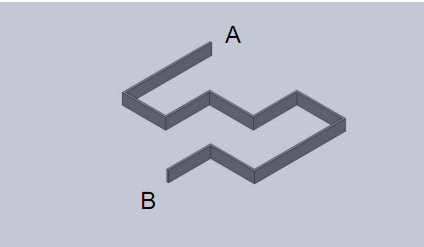
\includegraphics[width =  \textwidth]{graphics/course.png}
\cprotect \caption{Sample course layout for robotic wall-following.}
\label{course}
\end{minipage}
}
\end{figure}

The Amigobot is expected to navigate a course without collisions and
in a specified time frame. A sample course layout is shown in
Fig.~\ref{course}.

In addition to the required specifications, the wall following program
will improve the user interface of the robot by enhancing the
7-segment, LCD, and LED displays.

\subsection{Design Solution}

\subsubsection{Process and Sensor Description}

\begin{figure}[h!]
\centering
\cprotect \fbox{
\begin{minipage}{3.5in}
\centering
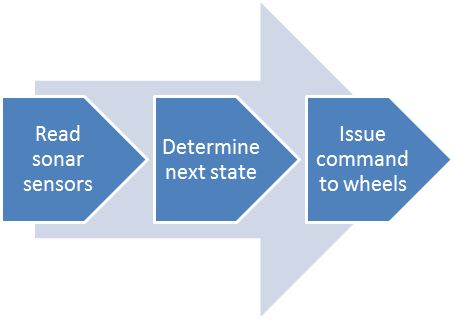
\includegraphics[width =  \textwidth]{graphics/flowchart.png}
\cprotect \caption{Flow chart of wall following algorithm.}
\label{flowchart}
\end{minipage}
}
\end{figure}

The wall following algorithm to be implemented follows the
process found in Fig.~\ref{flowchart}.

A switch will be used to toggle between following the left wall and
following the right wall.  The value of the switch determines which
sensors are actively collecting data. The values of the following
sensors will be used:
\begin{itemize}
\item Sensor \(s_0\) or \(s_5\):
\begin{itemize}
\item Measure the distance to the closest parallel wall (Fig.~\ref{s0s5}).
\item Measure lack of parallel wall by reading value greater than \verb+OT_THR+ (Fig.~\ref{s0s5t}).
\end{itemize}
\item Sensor \(s_2\) or \(s_3\):
\begin{itemize}
\item Measure the distance to approaching wall (Fig.~\ref{s2s3}).
\end{itemize}
\end{itemize}

\begin{figure}[h!]
\centering
\cprotect \fbox{
\begin{minipage}{3in}
\centering
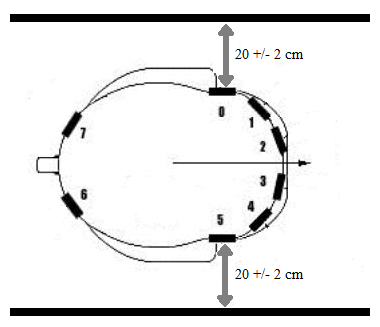
\includegraphics[width =  \textwidth]{graphics/s0s5.png}
\cprotect \caption{Sensors \(s_0\) and \(s_5\) measuring 
distance to wall.
}
\label{s0s5}
\end{minipage}
}
\end{figure}

\begin{figure}[h!]
\centering
\cprotect \fbox{
\begin{minipage}{2.5in}
\centering
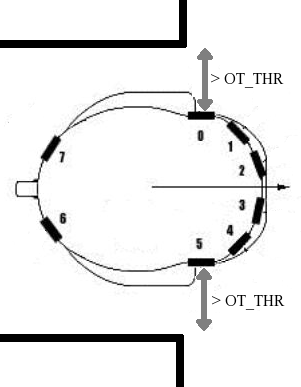
\includegraphics[width =  \textwidth]{graphics/s0s5t.png}
\cprotect \caption{Sensors \(s_0\) and \(s_5\) detecting outside corner.}
\label{s0s5t}
\end{minipage}
}
\end{figure}

\begin{figure}[h!]
\centering
\cprotect \fbox{
\begin{minipage}{3in}
\centering
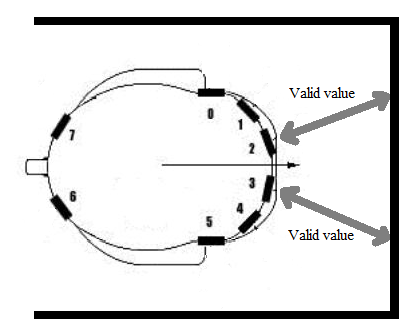
\includegraphics[width =  \textwidth]{graphics/s2s3.png}
\cprotect \caption{Sensors \(s_2\) and \(s_3\) measuring distance to front wall.}
\label{s2s3}
\end{minipage}
}
\end{figure}



\subsubsection{State Machine Description}
The description of the states is listed below. The UML state machine
diagram the team used to implement a solution is found in
Fig.~\ref{state}.

\begin{enumerate}
\item \textbf{Forward:} The robot will move forward alongside a
  wall. A tolerance of \(\pm2\) cm will be used to keep the robot in a
  range of 18-22 cm from the wall, measured by sensors
  \(s_0\) and \(s_5\).  If the robot is not in the specified range, it
  will switch to one of the adjustment states, which are dependent upon
  which wall is followed.  If a wall is detected in front of the robot
  by sensors \(s_2\) and \(s_3\), the robot will switch to the ``inside
  turn'' state. Likewise, if no wall is detected by sensors \(s_0\) and
  \(s_5\), the robot will switch to the ``outside turn'' state.
\item \textbf{Adjust Outward:} The robot veers slightly outwards to get
  back within the accepted distance range. After the robot is within
  the accepted distance range, the machine switches to the ``forward''
  state.
\item \textbf{Adjust Inward:} The robot veers slightly inwards to get
  back within the accepted distance range. After the robot is within
  the accepted distance range, the machine switches to the ``forward''
  state.
\item \textbf{Outside Turn:} The robot stops and turns \(90^\circ\) clockwise
  or counterclockwise, depending on if the wall followed is on the
  right side or on the left side. Fig.~\ref{ot} demonstrates this turn when
  the robot is following a right wall and is turning clockwise.
\item \textbf{Inside Turn:} The robot stops and turns \(90^\circ\) clockwise or
  counterclockwise, depending on if the wall followed is on the right
  side or on the left side. Fig.~\ref{it} demonstrates this turn when the
  robot is following a right wall and is turning counterclockwise.
\end{enumerate}

\begin{figure}[h!]
\centering
\cprotect \fbox{
\begin{minipage}{6.5in}
\centering
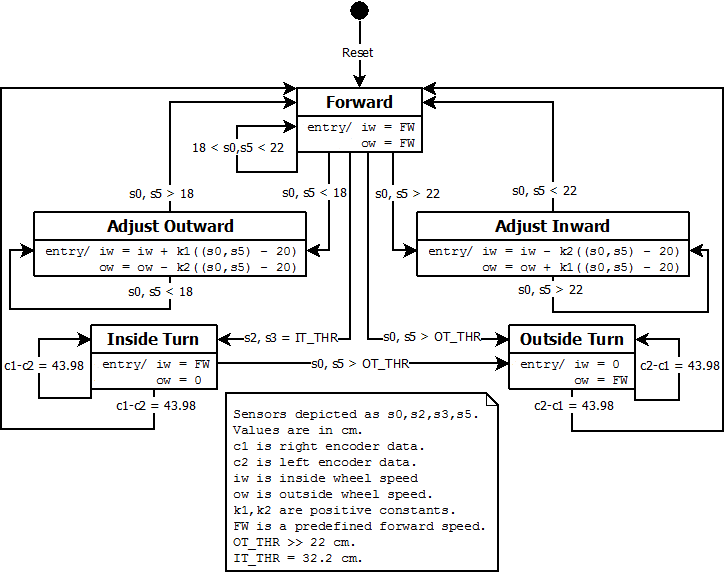
\includegraphics[width =  \textwidth]{graphics/state.png}
\cprotect \caption{UML state machine diagram for wall following algorithm for Amigobot.}
\label{state}
\end{minipage}
}
\end{figure}



\subsubsection{Turning}
The robot's turning algorithm takes advantage of the course only containing turns of approximately 90\(^\circ\). Such sharp turns
are not conducive towards ``smooth'' wall following techniques.
Therefore, when necessary, the robot will execute a blind turn which relies on the
optical rotary encoders on each wheel instead of the sonar data.
The goal of the turning algorithm is not to pivot exactly 90\(^\circ\)
and then move in a straight line every time, but rather to quickly execute a precise turn which results
in the robot being approximately parallel to and 20 cm away from the
opposite wall, after which the robot can easily continue using sonar
data to make accurate adjustments.

\paragraph{Detecting a Turn}
The turning algorithm being implemented requires accurate detection of
forward obstacles and discontinuities in the parallel wall in order to
avoid turning prematurely.

\begin{figure}[h!]
\centering
\cprotect \fbox{
\begin{minipage}{4in}
\centering
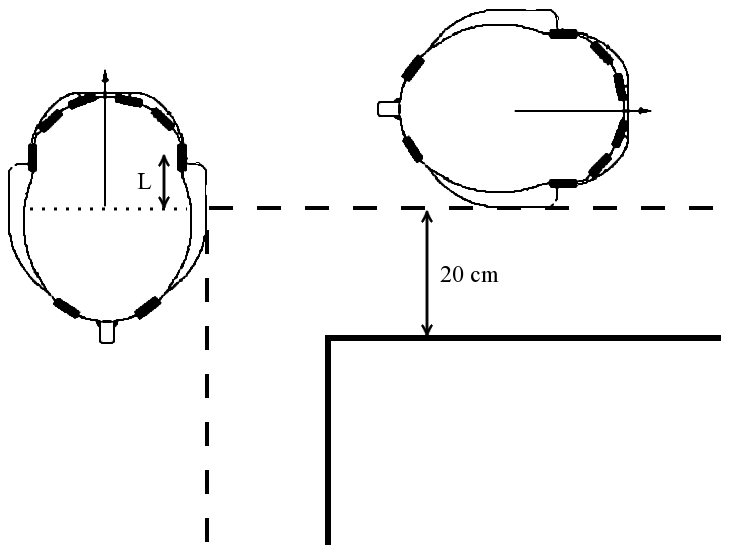
\includegraphics[width =  \textwidth]{graphics/outside_turn.png}
\cprotect \caption{Geometery of an outside turn. \(L\) represents
  the distance between the side sensor (\(s_0\) or \(s_5\)) and the
  wheel axis.}
\label{ot}
\end{minipage}
}
\end{figure}
The robot should execute an outside turn when it loses direct contact
with the parallel wall. This discontinuity occurs when the reading of
the horizontal sensor (\(s_0\) or \(s_5\)) jumps beyond some threshold
value \verb+OT_THR+, where \verb+OT_THR+ \(>> 22\) cm. Depending on
how reliable the sensor readings are, the data from these sensors may
need to be filtered with an averaging filter to prevent
premature turning. A diagram of the outside turn geometry is presented
in Fig.~\ref{ot}. Once the robot detects the absence of the parallel
wall, it will travel forward a distance of approximately 20 cm plus
\(L\), where \(L\) is the distance between the center of sensors
\(s_0\) or \(s_5\) and the wheel axis. After traveling forward, the
robot will execute a turn by driving the outside wheel at a positive
velocity while stopping the inside wheel until the robot has rotated
\(90^\circ\) (see \ref{exturn}), whereupon forward motion will
continue.

\begin{figure}[h!]
\centering
\cprotect \fbox{
\begin{minipage}{4in}
\centering
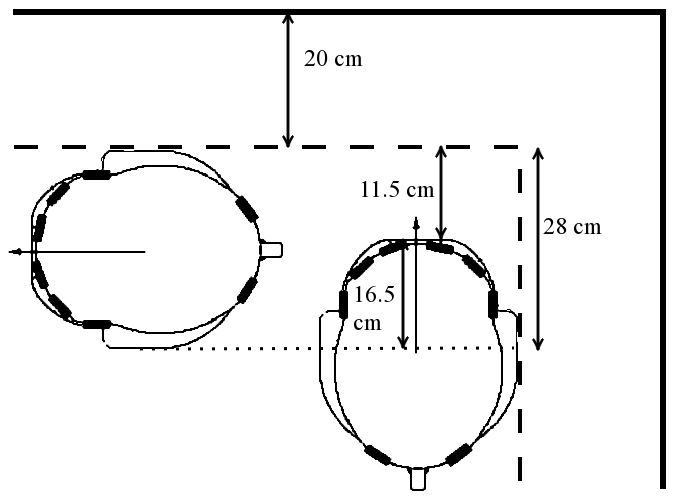
\includegraphics[width =  \textwidth]{graphics/inside_turn.png}
\cprotect \caption{Geometry of an inside turn.}
\label{it}
\end{minipage}
}
\end{figure}
For an inside turn, the robot must begin turning once the front of the
robot reaches the threshold \verb+IT_THR+. The geometry for this turn is
presented in Fig.~\ref{it}, which indicates that \verb+IT_THR+ should
be \(31.5\) cm. However, the forward sensors \(s_2\) and \(s_3\) are
not pointed directly forward, but rather are at \(12^\circ\) angles,
so the sensor reading for \verb+IT_THR+ should be
\(31.5/\cos(12^\circ)=32.2\) cm before the robot begins an inside
turn. 

The inside turn is executed in the same way as the outside turn;
the inside wheel is stopped while the outside wheel is driven forward
until the robot has rotated \(90^\circ\). However, while robot is
approaching a forward obstacle and preparing to turn, it is possible
 that the robot will encounter a discontinuity in the
parallel wall, indicating the actual necessity for an outside
turn. For this reason, while in the ``inside turn'' state the robot will
continue reading sensors \(s_0\) or \(s_5\) to detect if they exceed
\verb+OT_THR+. If at any point they do, the robot will transition from
making an inside turn to an outside turn as shown in the state
diagram (Fig.~\ref{state}).
\paragraph{Using the Rotary Encoders}
The optical rotary encoders on each wheel of the Amigobot provide an
incredibly fine yet robust way to detect the rotational position of
each wheel. Each wheel's position can be loaded through SCOMP's
I/O through the I/O addresses \verb+0x80+, \verb+0x81+, \verb+0x88+, and
\verb+0x89+, which respectively correspond to the given address names
\verb+LPOSLOW+, \verb+LPOSHIGH+, \verb+RPOSLOW+, and \verb+RPOSHIGH+. The position
datum from each encoder is a 32-bit number. For I/O purposes, this datum
is split into two 16-bit numbers (the upper 16 bits and the lower 16
bits), each of which corresponds to the ``low'' or ``high'' I/O
address for each wheel's position.

\paragraph{Physical Characteristics of the Rotary Encoders}
The encoder datum increments by \(39000\) for each revolution of the
wheel. The left encoder increments when the left wheel is in forward
motion, while the right encoder decrements when the right wheel is in
forward motion. Each wheel has a diameter of 10 cm, which results in a
path of 31.42 cm being traversed for each wheel revolution so long as
traction is maintained. Since there are \(39000\) ``ticks'' per
revolution, one cm of linear wheel motion corresponds to
\(1241.41\) ticks. This results in large-valued encoder data for
relatively short distances. In order to simplify calculations and
prevent bit carries between two 16-bit numbers (the high and low
data), it is best to perform calculations on a single 16-bit number
which can be produced by combining the upper eight bits of the ``low''
datum with the  lower eight bits of the ``high'' datum, resulting in a
reduction in encoder resolution by a factor of 256.  After shifting and truncating the two
16-bit numbers into one 16-bit number, the physical characteristics
of the encoder transform so that there are \(152.34\) ticks per wheel
revolution and \(4.85\) ticks per cm of linear wheel motion.

\paragraph{Executing a Turn}\label{exturn}
\begin{figure}[h!]
\centering
\cprotect \fbox{
\begin{minipage}{3.5in}
\centering
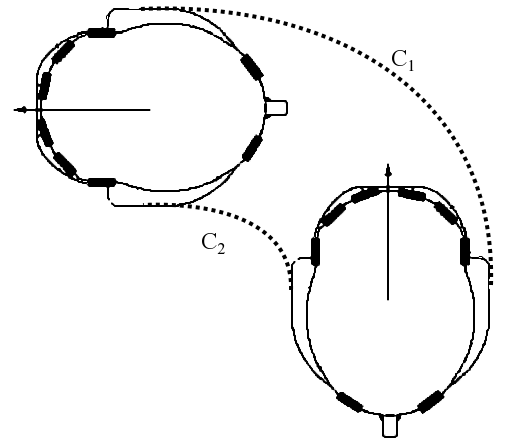
\includegraphics[width =  \textwidth]{graphics/turning.png}
\cprotect \caption{Path lengths \(C_1\) and \(C_2\) as the robot turns.}
\label{turning}
\end{minipage}
}
\end{figure}

The linear path lengths of each wheel are related by a constant such
that when the difference in path lengths of each wheel is equal to that
constant, the robot is oriented precisely at an angle \(\theta\) to its starting
orientation. If the robot has a wheel track of \(R\),
and the linear path lengths of the right and left wheels are
represented respectively by \(C_1\) and \(C_2\) (Fig.~\ref{turning}), then the robot has
turned positive (counterclockwise) \(\theta\) radians when the following equation is satisfied:
\begin{equation}
C_1 - C_2 = \theta R
\end{equation}
For instance, if the Amigobot (\(R = 28\) cm) is to turn about
90\(^\circ\) then continue forward, 
then the robot should cease turning when \(C_1-C_2 \geq 0.5\pi
(28) = 43.98\) cm, or about 213 (0x00D5) ticks. 

\subsubsection{Amigobot Display Additions}\label{xtras}
Several additions will be made to the robot display to improve the
user interface. Memory locations used to write to and read from are designated in capital letters. 
\begin{itemize}
\item Two displays will be used to show the velocity of the left and
  right wheels.
  \begin{itemize}
  \item These will be written to \verb+SEVENSEG+ whenever \verb+LVELCMD+ or \verb+RVELCMD+,
    the wheel velocities, are changed.
  \end{itemize}
\item The third display will show the velocity of the robot.
  \begin{itemize}
  \item This will be done by altering the \verb+IO_decoder+ and the
    block diagram
    files so that the second set of four 7-segment displays can be
    written. It will be called \verb+SEVENSEG2+ and mapped to 0x05 on the
    IO address space map.
  \item\verb+IO_decoder+ will be altered by adding and enabling a signal
    for the second set of the 7-segment LEDs and copying the setup of
    the \verb+HEX_DISP+ module used for the current 7-segment display.
  \end{itemize}
\item The LCD display will show the current state. The state name will
  either be encoded or spelled out on the display.
  \begin{itemize}
  \item This will be done by altering the LCD display to accept ASCII
    values representing numbers. The SLCD will be altered to take in
    an ASCII enable, \verb+ASCII_EN+, which will tell it to interpret the
    incoming argument as a state to be output in ASCII format.
  \item The states will be encoded into a binary code of 16 bits. For
    example, the ``forward'' state would be encoded as 0x0 and the
    ``adjust left'' state as
    0x1. The strings shown on the LCD display will be hard coded using
    the binary state representations.
  \end{itemize}
\item The red LEDs will light up to show the progress of a turn as the
  robot is turning.
  \begin{itemize}
  \item The red LED I/O has already been implemented in
    SCOMP at I/O address space 0x01.
  \end{itemize}
\item The green LEDs will be used to display a pattern unique to the state that the robot is in.
  \begin{itemize}
  \item This will be done by altering the \verb+IO_decoder+ and the BDF
    files so that the green LEDs can be used. It will be called GLEDS
    and mapped to 0x07 on the IO address space map.
  \end{itemize}
\end{itemize}










\section{Management Plan}
The design will be executed according to the Gantt chart provided in Appendix A. 

\subsection{Contingency Plan}
In the event that the team cannot complete all tasks before the
deadline, the team will implement the state machine with the states 
``forward,''  ``adjust inward,'' ``adjust outward,'' ``inside turn,'' and
``outside turn.'' These requirements are fundamental to the wall following 
solution algorithm. Additional features outlined in \ref{xtras} will 
be implemented as time and resources permit.  

In the event that the presented algorithm does not adequately provide
a means for the Amigobot to follow a wall, a different, slower, and smoother
algorithm will be implemented. This backup program will eliminate the
need for the ``outside turn'' state and adjustment states, instead
continuously and smoothly adjusting the wheel velocities in forward
motion depending on
how far the robot is from the parallel wall. When there is a parallel
wall discontinuity, the measured distance will jump high and the robot
will adjust by increasing the outside wheel velocity, effectively
turning automatically. Inside turns will be accomplished by stopping
the robot when it is close to a forward obstacle, then rotating in
place until the front sensor, \(s_2\) or \(s_3\), no longer detects a
forward obstacle, whereupon forward motion will continue.

\titleformat{\section}{\LARGE\bfseries}{\appendixname\:\thesection:}{1em}{}{}

\newpage
\begin{appendices}
%\appendixtitleon
%\appendixname
\section{Gantt Chart}
\begin{center}
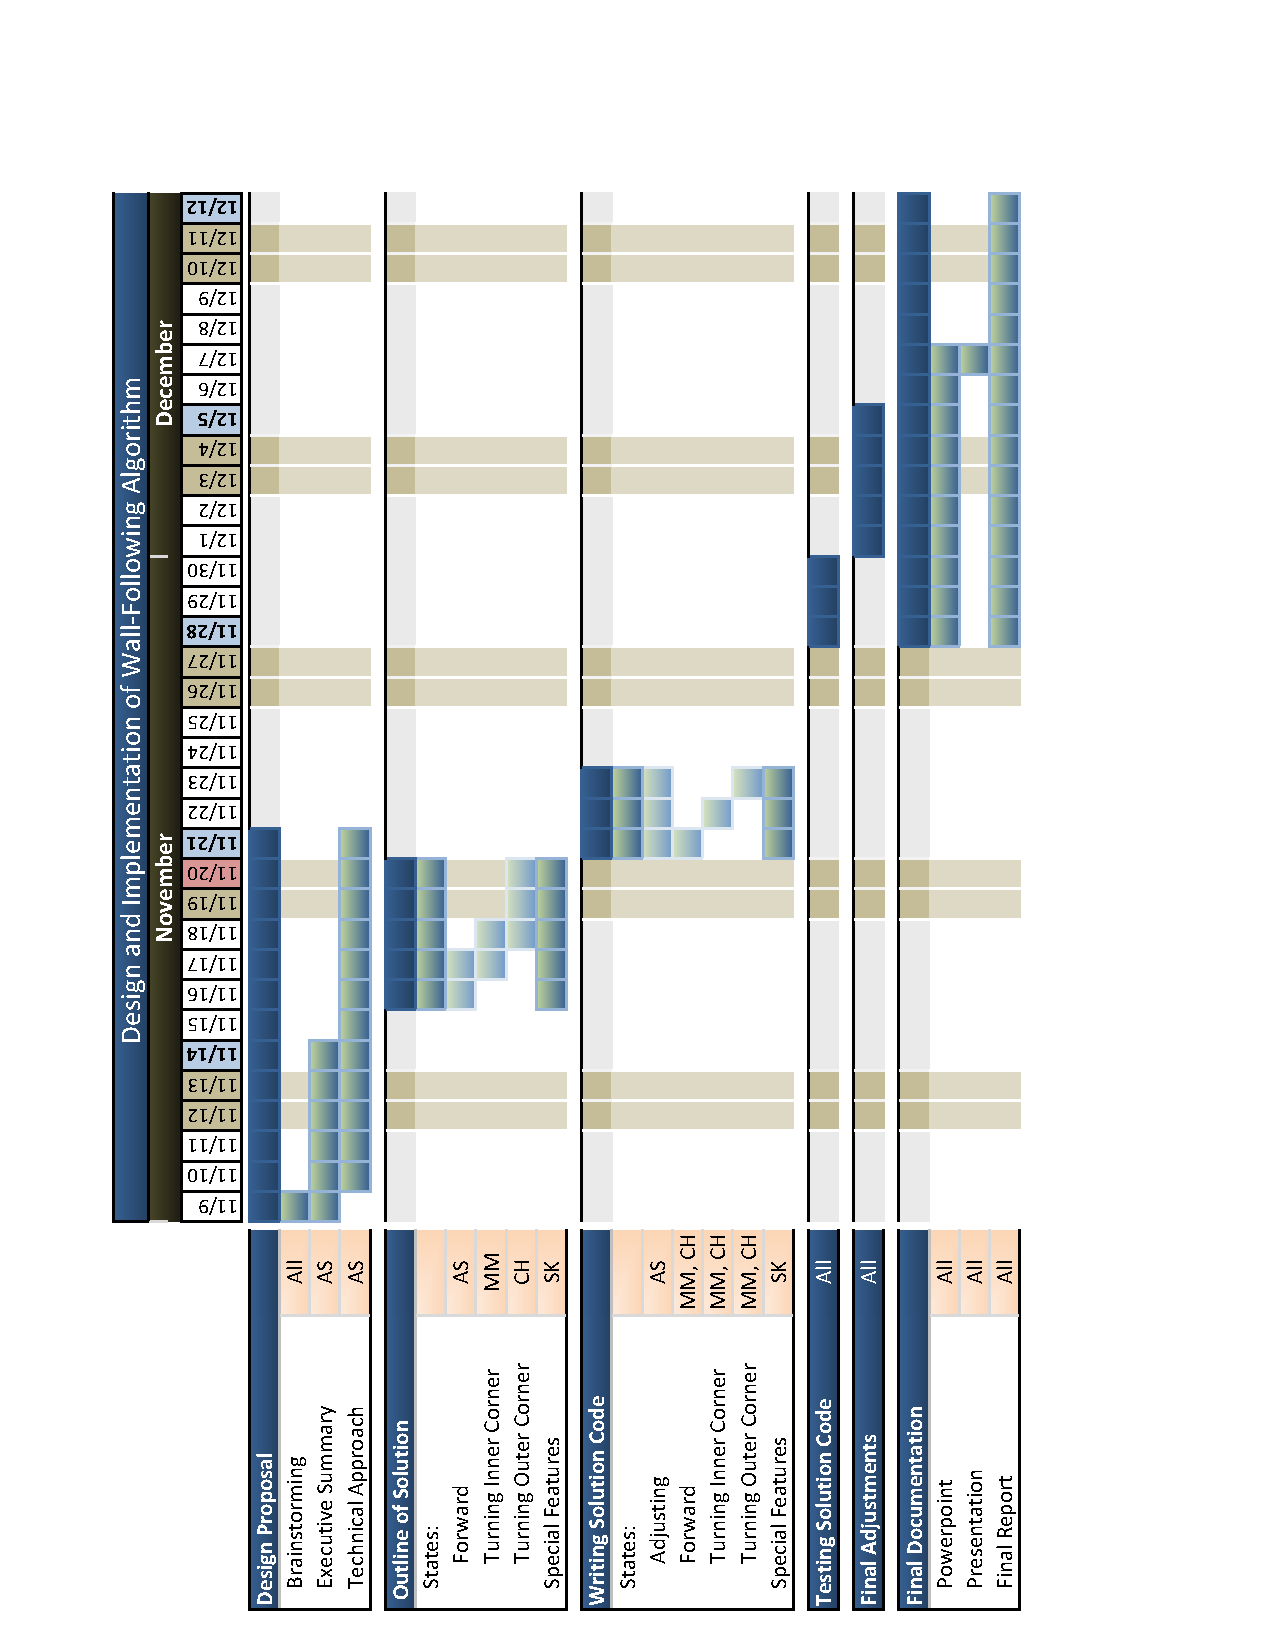
\includegraphics[height = 8in]{graphics/gantt_chart}
\end{center}
\end{appendices}


%\bibliographystyle{IEEEtran}
%\bibliography{IEEEabrv,bib-1}

\end{document}



%\begin{figure}[h!]
%\centering
%\cprotect \fbox{
%\begin{minipage}{6.5in}
%\centering
%\includegraphics[width =  \textwidth]{img_here}
%\cprotect \caption{}
%\end{minipage}
%}
%\end{figure}

